%%%%%%%%%%%%%%%%%%%%%%%%%%%%%%%%%%%%%%%%%%%%%%%%%%%%%%%%%%%%%%%%%%%%%%%%%%%%%%%%%%%%%%%%%%
\section{Evaluation}
%%%%%%%%%%%%%%%%%%%%%%%%%%%%%%%%%%%%%%%%%%%%%%%%%%%%%%%%%%%%%%%%%%%%%%%%%%%%%%%%%%%%%%%%%%i

\subsection{Security: do we meet our meet security goals}
   - attack scenarios

\subsection{Performance}
\begin{table}
\begin{center}
\begin{tabular}{ c c }
 \textbf{High-Level Operation} & \textbf{Time (mus)}\\
    Single User GDPR Deletion & \\
    Single User GDPR Restore & \\
    Single User Anonymization & \\
    Edit Anonymized Lecture& \\
    Create Account & \\
\hline
    \textbf{DB Operation} & \textbf{Time (mus)}\\
\hline
Insert DB Row (User )& 120\\
Update DB Row (FK) & 64\\ 
Select DB Row (User) & 120\\
Remove DB Row (User) & 90\\
Select DB Rows (Answers) & 160\\
Remove DB Rows (Answers) & 150\\
Reveal Deleted Row (DB Select + Insert) & 160 \\
Create + Register Principal & 110\\
\hline
    \textbf{Crypto Operation} & \textbf{Time (mus)}\\
\hline
Generate Keypair & 300831\\
Encrypt Ownership Token & 360\\
Decrypt Ownership Token & 3000\\
Encrypt Diff Token & 340\\
Decrypt Diff Token & 3000\\
\end{tabular}
\end{center}
\caption{Amount of time required to run different operations for disguises in WebSubmit}
\end{table}


   1) Normal operation: overheads imposed by Edna
    1.1) Cost of pseudoprincipals
         - Query runtime
         - Storage space
   2) Disguise operations
    2.1) Impact on concurrent users of web app
    2.2) Latency of the operations themselves

\subsection{Case studies}
   1) websubmit
      - was Edna sufficient for the application's needs?
      - changes to application required (how much work to integrate Edna?)
      - *how* did application use Edna?
        - what disguises?
        - how caps integrated with application?
   2) HotCRP
   3) Lobsters?

\begin{figure*}[t!]
    \centering
    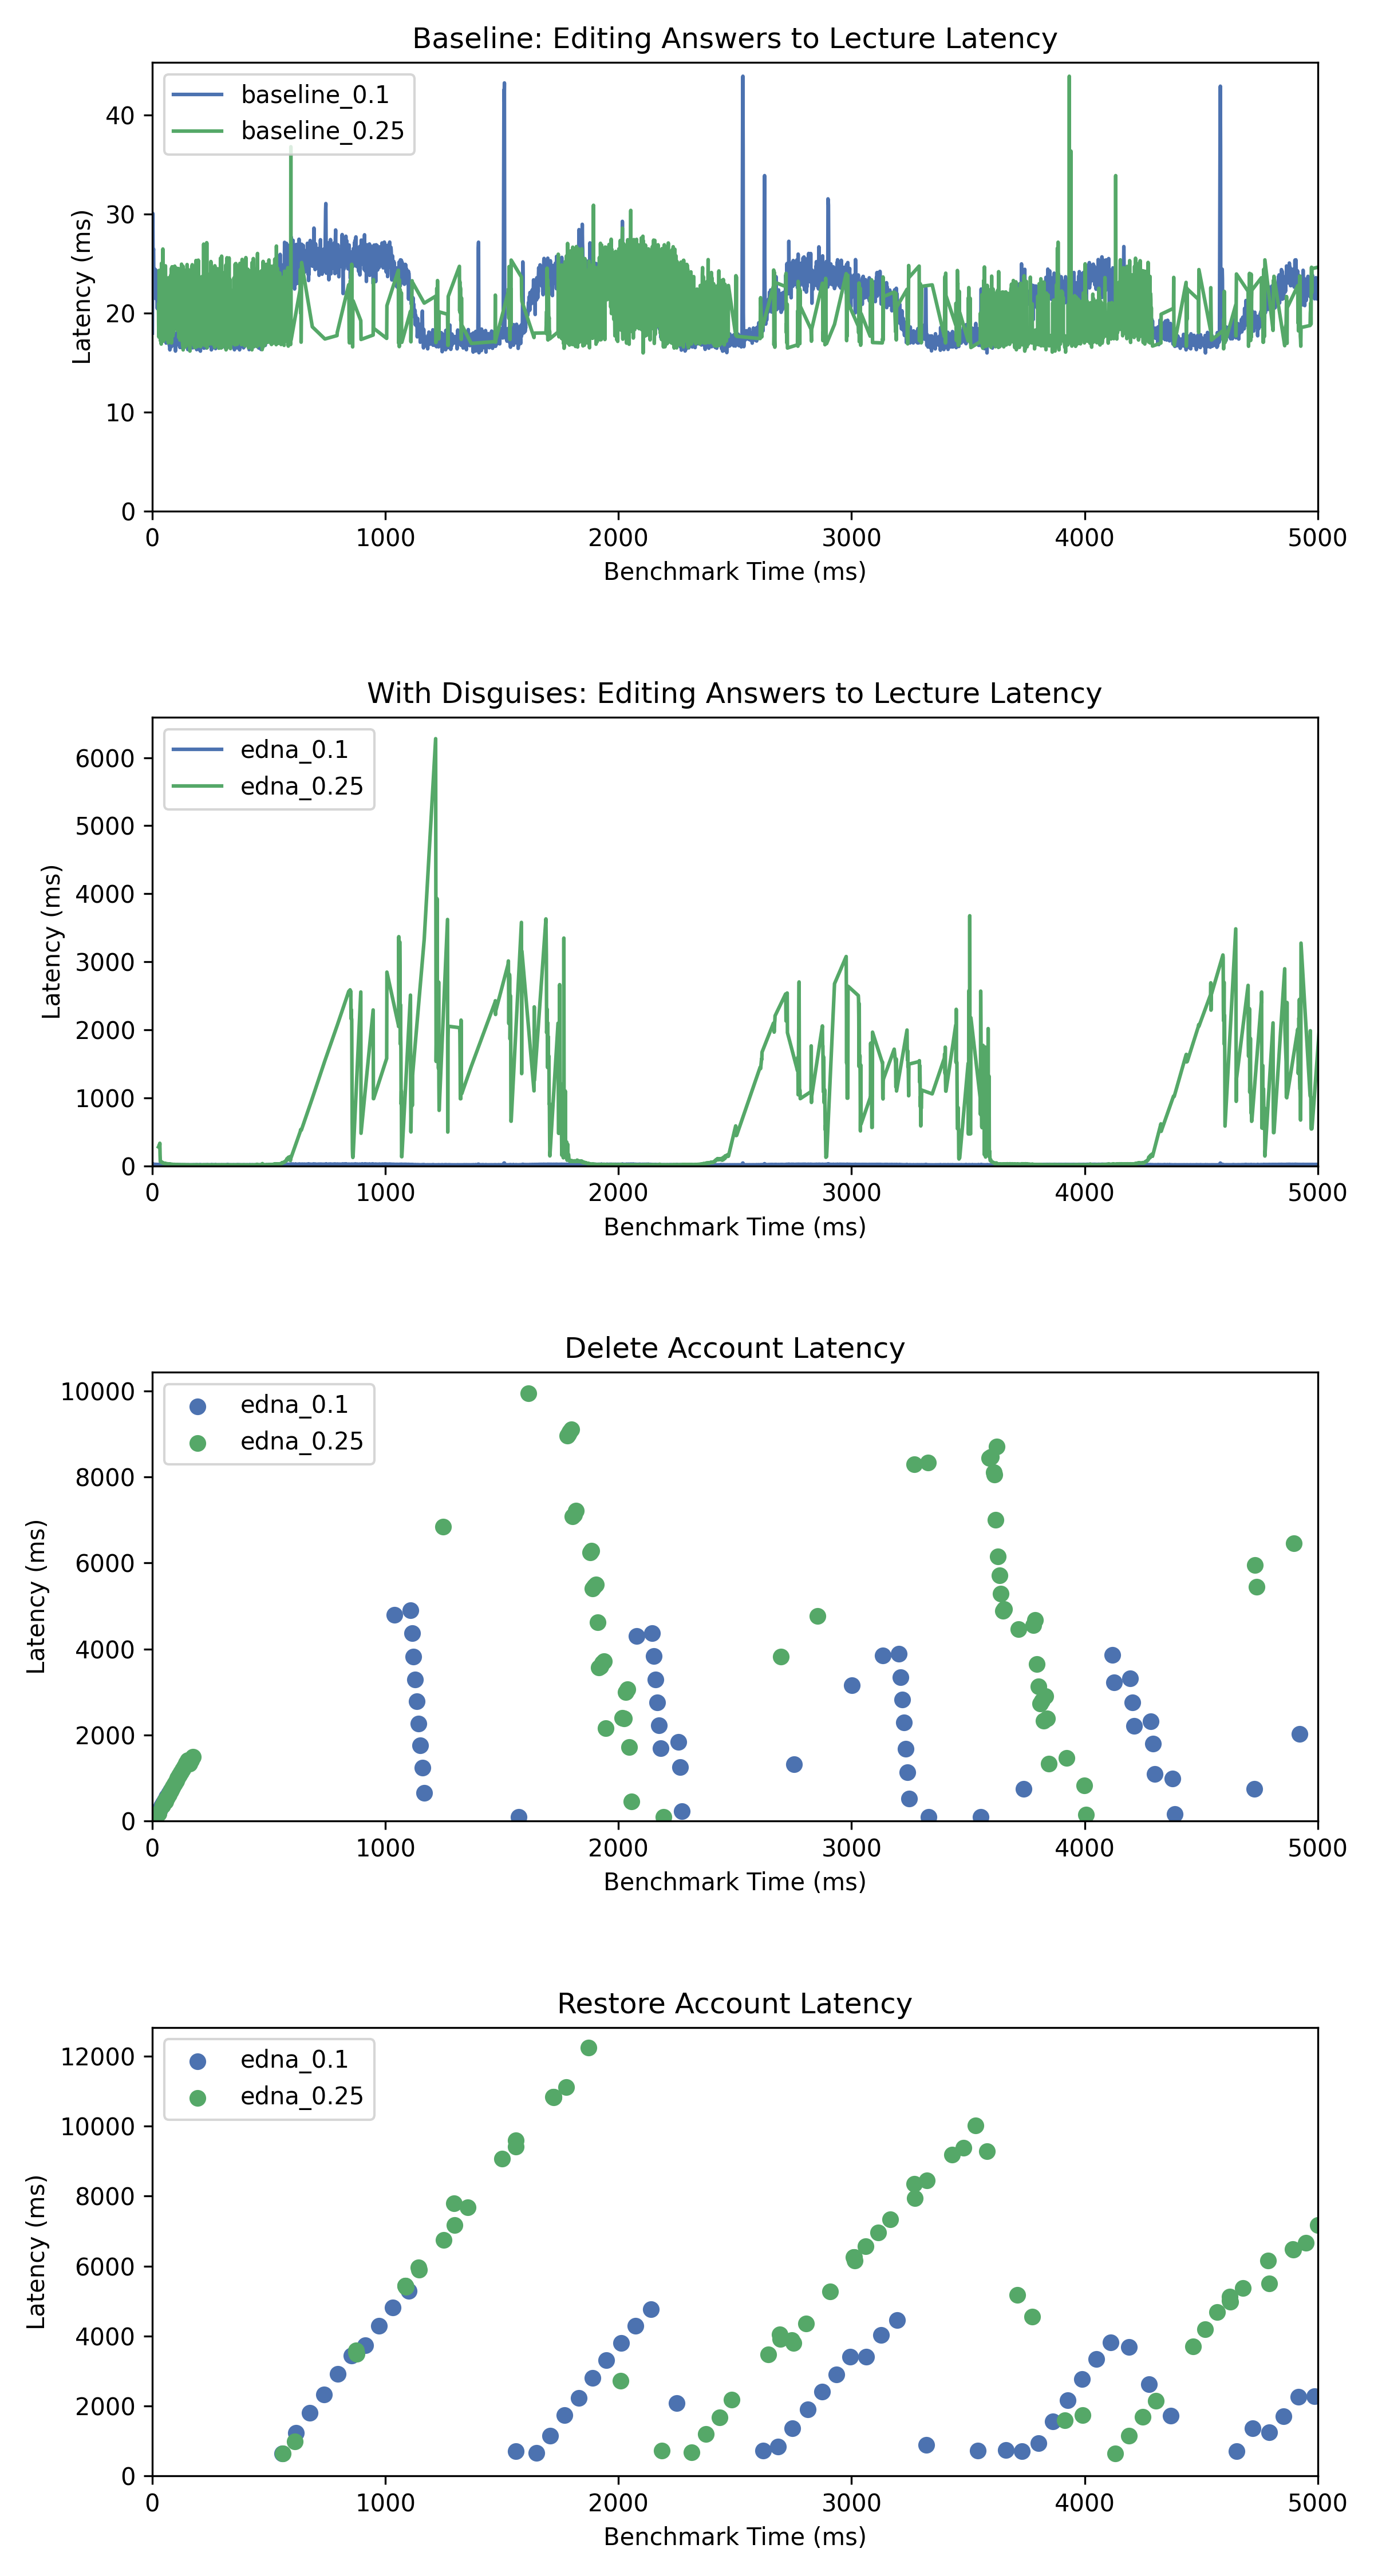
\includegraphics[width=0.45\textwidth]{figs/concurrent_results_40lec_100users}
    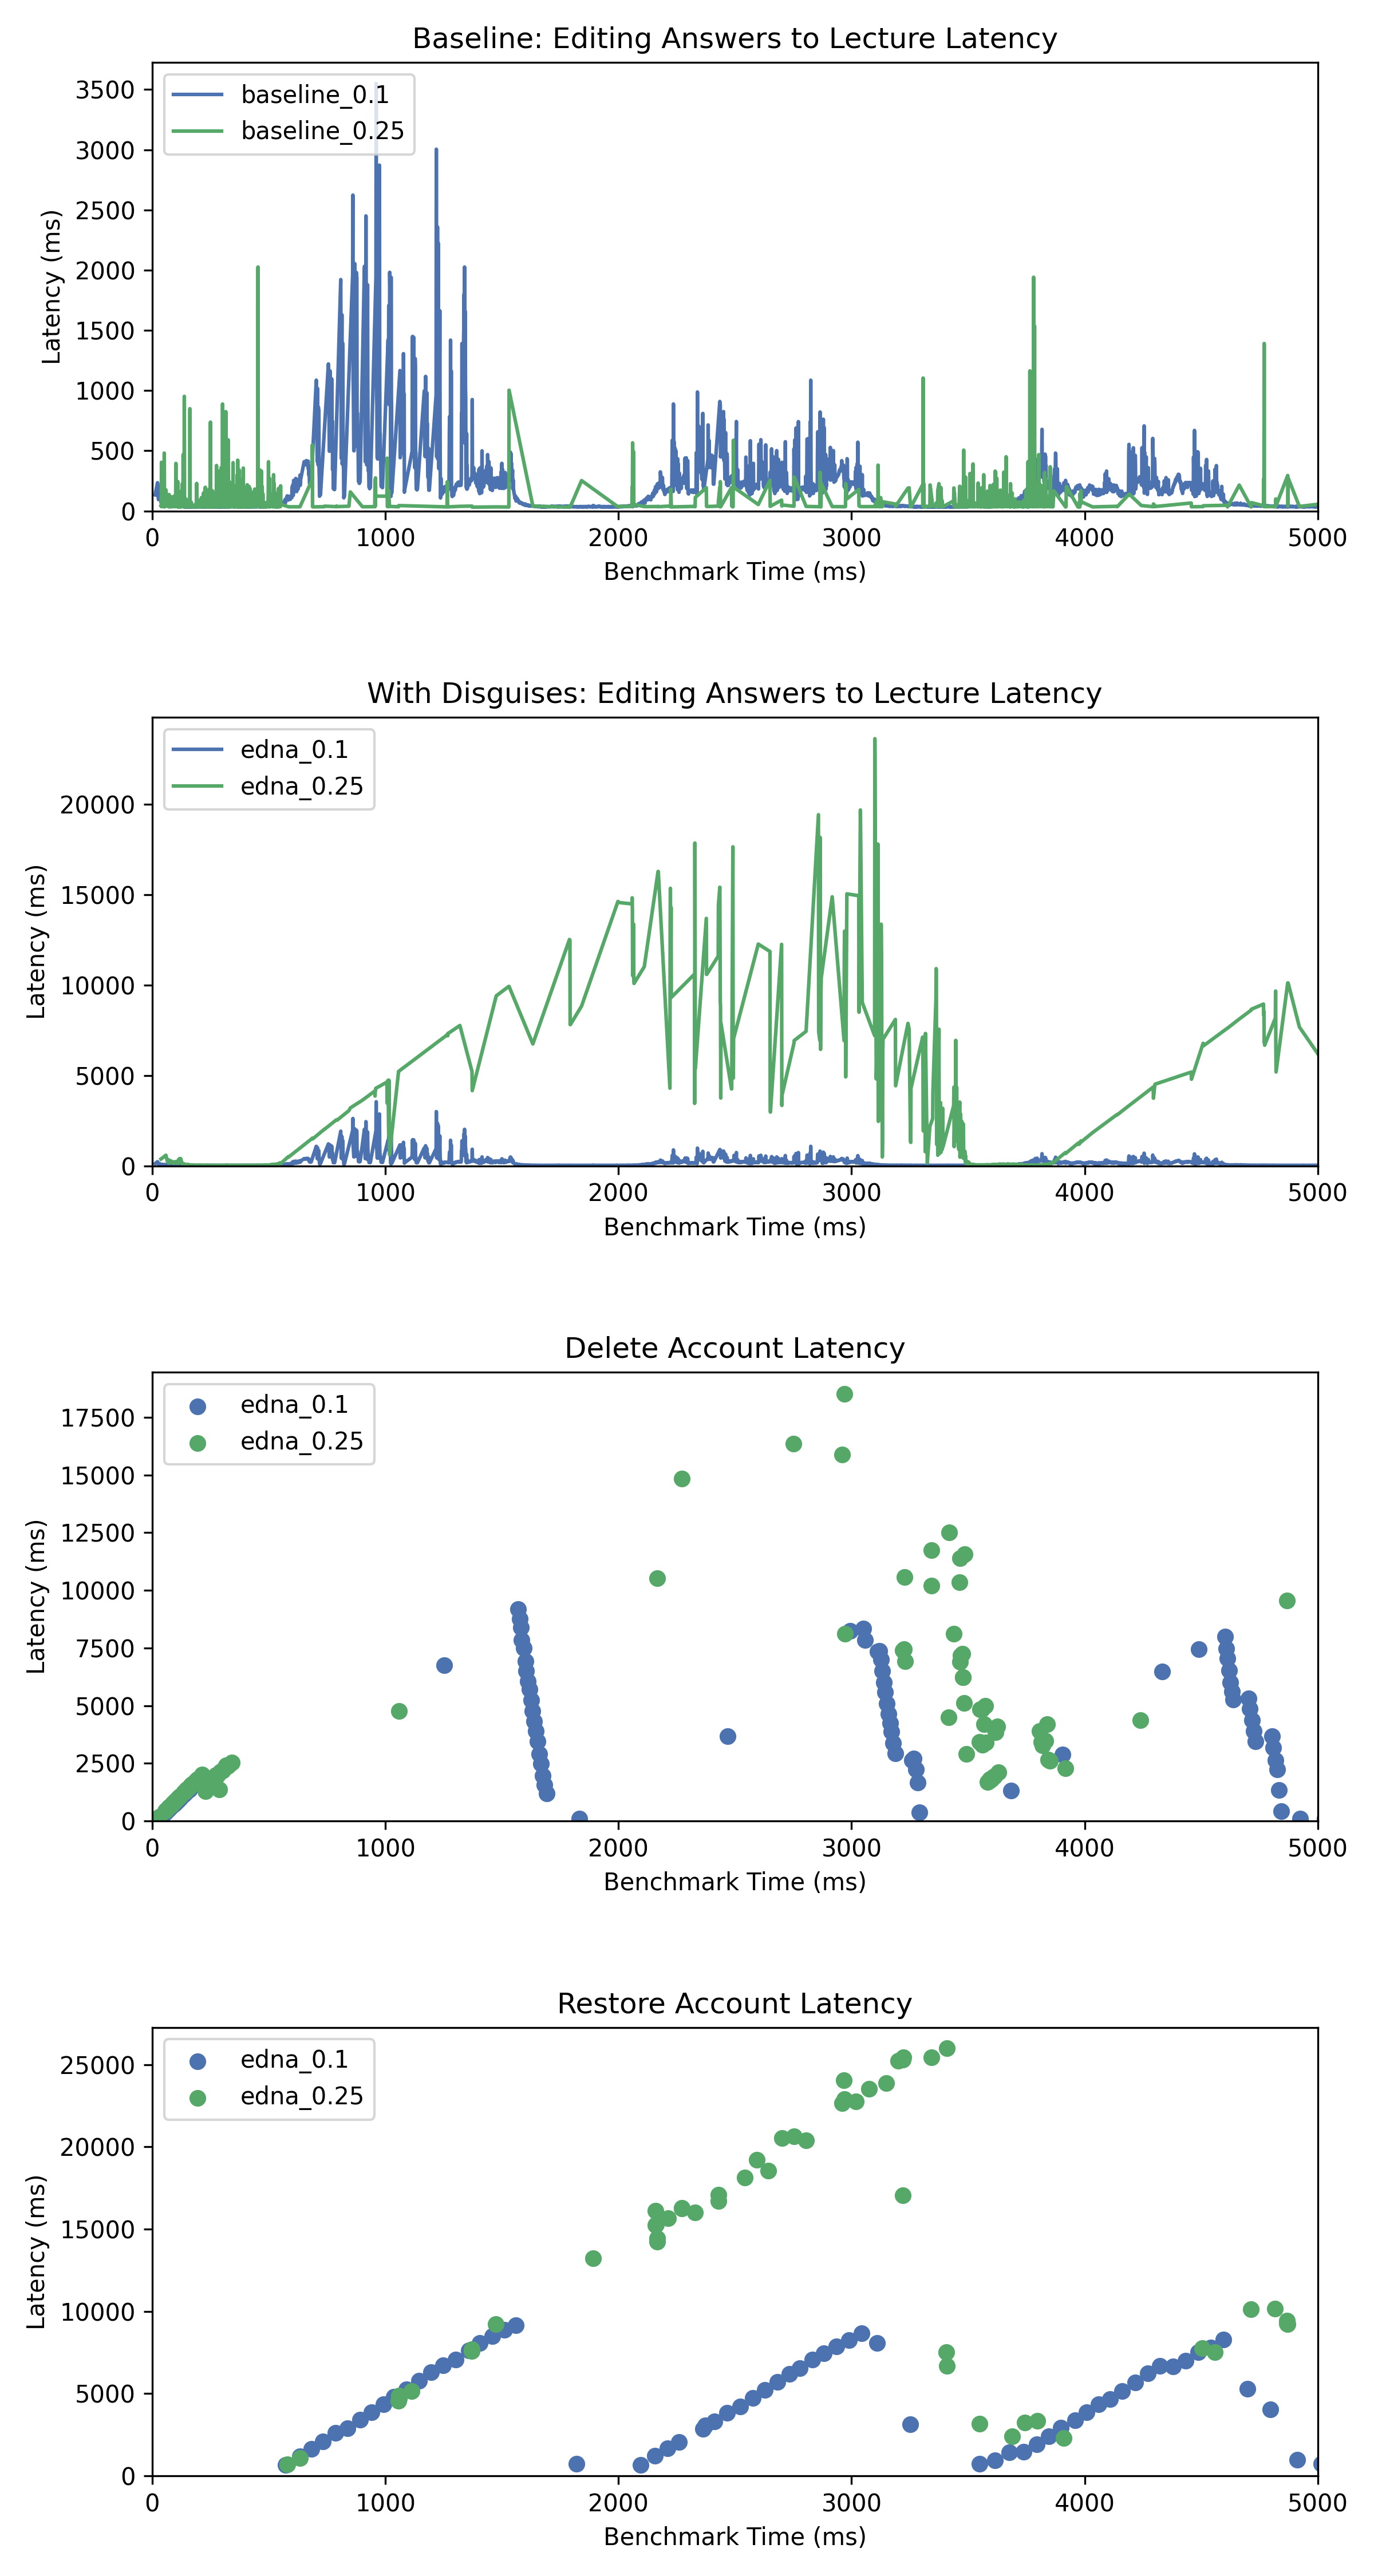
\includegraphics[width=0.45\textwidth]{figs/concurrent_results_40lec_200users}
    \caption{100 Users (left), 200 users (right); 
    40 lectures; 4 questions/lecture; ~5s sleep between disguise and reveal. }
\end{figure*}
